\chapter{Representations of 3D Shapes}\label{ch:repr}

A 3D shape can be stored in many ways, and the choice decides which operations are cheap. A
scanner produces points, a physician receives a voxel volume, a designer edits spline patches, a
GPU draws triangles, and many modern algorithms prefer a function whose zero level set is the
surface. This chapter reviews the main representations, their strengths and costs, and the
conversions between them (\cref{fig:repr}). The companion notebook builds each one in Python.

\fig{ch02_representations.png}{The same object (the Stanford bunny) in five representations: an
oriented point cloud, a coarse triangle mesh, an occupancy voxel grid, a slice of a signed
distance function $f$ (blue inside, red outside, black zero level) and the mesh extracted from
$\{f=0\}$ by marching cubes.}{fig:repr}

\section{A taxonomy}

Two distinctions organise the zoo of representations.
\begin{itemize}
  \item \textbf{Surface versus volume.} A boundary (surface) representation stores only the
  interface between inside and outside: point clouds, meshes, parametric patches. A volumetric
  representation describes the whole space: voxel grids, octrees, implicit functions.
  \item \textbf{Explicit versus implicit.} An explicit representation lists or generates points of
  the surface, for example a parameterization $\bx(u,v)$ or the vertices of a mesh. An implicit
  representation gives a test: $\bx$ is on the surface if $f(\bx)=0$. Explicit forms make sampling
  and rendering easy; implicit forms make inside/outside queries, Boolean operations and changes of
  topology easy.
\end{itemize}

\begin{table}[tbp]
\centering\small
\begin{tabularx}{\textwidth}{@{}lXXX@{}}
\toprule
Representation & Strengths & Weaknesses & Typical source \\
\midrule
Point cloud & raw sensor output; trivial to store and transform & no connectivity, no
inside/outside, needs neighbourhood search & scanners, photogrammetry \\
Voxel grid & regular, trivial Boolean operations, convolution & memory $O(n^3)$, blocky,
resolution bound & CT/MRI, simulation, 3D CNNs \\
Parametric patch & smooth, compact, exact derivatives & topology fixed by the patch layout,
trimming, stitching & CAD (NURBS) \\
Triangle mesh & universal, GPU friendly, arbitrary topology & piecewise linear, quality
dependent operators & modelling, reconstruction \\
Implicit (SDF) & inside/outside, Booleans, topology changes free & surface not explicit,
extraction needed & reconstruction, modelling, neural fields \\
\bottomrule
\end{tabularx}
\caption{Overview of the representations discussed in this chapter.}
\label{tab:repr}
\end{table}

\section{Point clouds}\label{sec:pointclouds}

A point cloud is a finite set $P=\{\bp_i\}_{i=1}^n\subset\R^3$, optionally with attributes per
point such as a normal $\bn_i$, a colour or a confidence. In code it is simply an $n\times 3$ array.
Point clouds are the natural output of 3D scanners (\cref{ch:acq}) and the input of registration
and reconstruction. They carry no connectivity, so every geometric operation starts with a
neighbourhood query.

\subsection{Sampling a mesh}

To produce a point cloud from a mesh with uniform density with respect to area, pick a triangle
with probability proportional to its area and then a uniform point inside it. If $r_1,r_2\sim
U(0,1)$, the point
\begin{equation}
\bp=(1-\sqrt{r_1})\,\bx_a+\sqrt{r_1}(1-r_2)\,\bx_b+\sqrt{r_1}\,r_2\,\bx_c
\label{eq:triangle-sampling}
\end{equation}
is uniformly distributed in the triangle $(\bx_a,\bx_b,\bx_c)$. The square root compensates for the
fact that the segment at ``height'' $s$ from vertex $a$ has length proportional to $s$: the
density of $s=\sqrt{r_1}$ is $2s$, which is exactly the length weight.

Uniform random samples cluster and leave gaps. \emph{Poisson-disk} (blue noise) sampling enforces a
minimum distance $r$ between samples, which gives an even coverage with the same number of points
(\cref{fig:sampling}); a simple implementation draws a dense uniform sample and eliminates every
point closer than $r$ to an accepted one \citep{Bridson2007}. \emph{Voxel downsampling} replaces
the points that fall in each cell of a grid by their average and is the standard way to thin a
dense scan.

\fig{ch02_sampling.png}{Uniform random sampling versus Poisson-disk sampling of the bunny with
3000 points each. The histogram of nearest-neighbour distances shows the difference: random
samples have many very close pairs, while the Poisson-disk sample has none below the radius
$r=0.0128$ (unit bounding-box diagonal).}{fig:sampling}

\subsection{Neighbourhood queries and kd-trees}

Normal estimation, ICP, outlier removal and reconstruction all ask for the $k$ nearest neighbours
of a point or for all points within a radius. Brute force costs $O(n)$ per query and $O(n^2)$ for
all points. A \emph{kd-tree} \citep{Bentley1975,Friedman1977} partitions space recursively with
axis-aligned planes:
\begin{enumerate}
  \item choose a splitting axis (cycling $x,y,z$, or the axis of largest spread);
  \item split at the median coordinate, so both children hold half of the points;
  \item recurse until a leaf holds at most a few points.
\end{enumerate}
Construction costs $O(n\log n)$ with linear-time median selection, and the tree has depth
$O(\log n)$. A \emph{range query} descends only into cells that intersect the query box or ball. A
\emph{nearest-neighbour query} descends to the leaf containing the query, records the best
distance $d^\star$, and on the way back visits the other child of a node only if the splitting
plane is closer than $d^\star$; for $k$ neighbours $d^\star$ is the distance to the current
$k$-th best, kept in a max-heap. In low dimension the expected cost is $O(\log n)$ per query
(\cref{fig:kdtree,fig:kdbench}); in high dimension the pruning test rarely succeeds and the search
degenerates to brute force, which is why \cref{ch:fmaps} uses dense matrix products for
nearest neighbours in 100-dimensional spectral spaces.

\fig{ch02_kdtree.png}{A 2D kd-tree. Left: the cells produced by recursive median splits. Centre:
a range query visits only the cells that intersect the query rectangle (highlighted). Right: a
$k$-nearest-neighbour query ($k=6$).}{fig:kdtree}

\fign{ch02_kdtree_bench.pdf}{Time per query of brute force (linear in $n$) and of a kd-tree
(nearly constant), and the build time divided by $n$ (growing like $\log n$), measured with
\texttt{scipy.spatial.cKDTree} on uniform points.}{fig:kdbench}

\section{Volumetric representations}

\subsection{Voxel grids}

A voxel grid divides a bounding box into $n^3$ cubic cells and stores a value per cell: a binary
occupancy, a density (CT scans), a signed distance, or a feature vector (3D convolutional
networks). The grid is trivially indexed, neighbours are implicit, and Boolean operations are
cell-wise logical operations. The price is memory: a $512^3$ grid of floats needs 512\,MB, while
the surface only intersects $O(n^2)$ cells. Coarse grids make the shape blocky
(\cref{fig:voxels}). A surface voxelization marks the cells that contain surface points; a solid
voxelization also fills the interior, for example by casting a ray along each grid column and
toggling inside/outside at every surface crossing (parity rule). The volume of a solid is then
approximated by the number of occupied cells times the cell volume.

\fig[0.8\textwidth]{ch02_voxel_resolution.png}{Surface voxelization of the bunny at resolutions
$n=12,24,48$. The occupied cells are $432$, $1832$ and $7437$, that is $25\%$, $13\%$ and $6.7\%$ of
the $n^3$ cells: the count grows like $n^2$ and the fraction decreases like $1/n$, which motivates
sparse and adaptive grids.}{fig:voxels}

\subsection{Adaptive grids}

Because the interesting cells concentrate near the surface, adaptive structures refine only
there. An \emph{octree} splits a cell into eight children when it contains surface; memory becomes
proportional to the surface area. OpenVDB \citep{Museth2013} uses a shallow tree with large
fan-out (for example $32^3$, $16^3$ and $8^3$ nodes) similar to a B+tree, giving fast random
access, sparse storage of a narrow band around the surface, and dynamic topology, and it is the
industry standard for level sets in visual effects.

\section{Surfaces and manifoldness}

\begin{definition}[2-manifold]
A surface $S\subset\R^3$ is a \emph{2-manifold} if every point has a neighbourhood homeomorphic to
an open disk. It is a 2-manifold with boundary if every point has a neighbourhood homeomorphic to
a disk or to a half-disk.
\end{definition}

For a triangle mesh, manifoldness reduces to two combinatorial conditions: every edge is shared by
one (boundary) or two (interior) triangles, and the triangles around every vertex form a single
fan, closed for interior vertices and open for boundary vertices (\cref{fig:nonmanifold}). A
surface is \emph{orientable} if a consistent normal direction can be chosen; for meshes this means
the faces can be ordered so that every interior edge is traversed in opposite directions by its two
faces. Most algorithms in these notes assume oriented 2-manifold meshes, and data structures such as
the half-edge (\cref{ch:ds}) cannot even represent non-manifold configurations.

\begin{figure}[tbp]
\centering
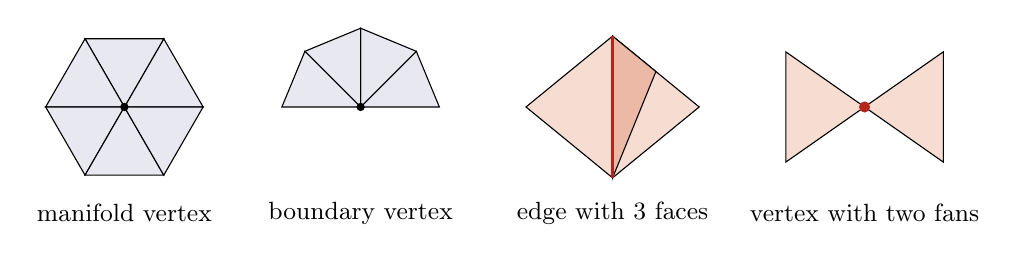
\begin{tikzpicture}[scale=1.0, every node/.style={font=\small}]
  % manifold interior vertex
  \begin{scope}
    \foreach \a in {0,60,...,300} {\draw[fill=MidnightBlue!10] (0,0) -- (\a:1) -- (\a+60:1) -- cycle;}
    \fill (0,0) circle (1.5pt);
    \node at (0,-1.35) {manifold vertex};
  \end{scope}
  % boundary vertex
  \begin{scope}[xshift=3cm]
    \foreach \a in {0,45,90,135} {\draw[fill=MidnightBlue!10] (0,0) -- (\a:1) -- (\a+45:1) -- cycle;}
    \fill (0,0) circle (1.5pt);
    \node at (0,-1.35) {boundary vertex};
  \end{scope}
  % non-manifold edge
  \begin{scope}[xshift=6.2cm]
    \draw[fill=BrickRed!12] (0,-0.9) -- (0,0.9) -- (-1.1,0) -- cycle;
    \draw[fill=BrickRed!12] (0,-0.9) -- (0,0.9) -- (1.1,0) -- cycle;
    \draw[fill=BrickRed!25] (0,-0.9) -- (0,0.9) -- (0.55,0.45) -- cycle;
    \draw[very thick, BrickRed] (0,-0.9) -- (0,0.9);
    \node at (0,-1.35) {edge with 3 faces};
  \end{scope}
  % non-manifold vertex (bow tie)
  \begin{scope}[xshift=9.4cm]
    \draw[fill=BrickRed!12] (0,0) -- (-1,0.7) -- (-1,-0.7) -- cycle;
    \draw[fill=BrickRed!12] (0,0) -- (1,0.7) -- (1,-0.7) -- cycle;
    \fill[BrickRed] (0,0) circle (2pt);
    \node at (0,-1.35) {vertex with two fans};
  \end{scope}
\end{tikzpicture}
\caption{Manifold and non-manifold configurations. Left: the neighbourhood of a manifold vertex is
a disk (interior) or half-disk (boundary). Right: an edge shared by three triangles and a vertex
whose triangles form two separate fans are non-manifold.}
\label{fig:nonmanifold}
\end{figure}

\section{Parametric surfaces}

A parametric surface is a map $\bx:\Omega\subset\R^2\to\R^3$, $(u,v)\mapsto\bx(u,v)$. Sampling is
immediate, and derivatives $\bx_u,\bx_v$ are available in closed form, so normals and curvatures
are exact (\cref{ch:diffgeo}). The difficulty is global: a single patch has the topology of its
domain, so a complex object needs many patches whose boundaries must be stitched with continuity
conditions.

\paragraph{B\'ezier curves and patches.} The Bernstein polynomials
$B_i^n(t)=\binom{n}{i}t^i(1-t)^{n-i}$ are non-negative and sum to one. A B\'ezier curve with
control points $\bc_0,\dots,\bc_n$ is $\bx(t)=\sum_i B_i^n(t)\bc_i$: it interpolates the end
points, is tangent to the control polygon there, and lies in its convex hull. The tensor-product
patch
\begin{equation}
\bx(u,v)=\sum_{i=0}^{m}\sum_{j=0}^{n}B_i^m(u)\,B_j^n(v)\,\bc_{ij}
\end{equation}
is controlled by a grid of points (\cref{fig:parametric}). \emph{B-splines} replace the global
Bernstein basis by piecewise polynomials with local support, so moving a control point changes the
surface only nearby, and \emph{NURBS} (non-uniform rational B-splines) add weights,
$\bx(u)=\sum_i w_iN_i(u)\bc_i/\sum_iw_iN_i(u)$, which allows exact conics such as circles. NURBS are
the standard of CAD; the slides of Tema 8 contrast them with triangle meshes: NURBS are compact and
smooth but need trimming curves and stitching for complex topology, whereas meshes handle
arbitrary topology uniformly.

\fig[0.95\textwidth]{ch02_parametric.png}{Left: a bicubic B\'ezier patch and its $4\times4$
control net; the patch interpolates the four corner control points. Right: a torus generated by
sampling $\bx(u,v)=((R+r\cos v)\cos u,(R+r\cos v)\sin u,r\sin v)$ on a periodic $(u,v)$ grid and
connecting neighbouring samples; the mesh has Euler characteristic $0$.}{fig:parametric}

\section{Triangle meshes}

A triangle mesh $\M=(V,E,F)$ consists of vertices with positions $\bx_i\in\R^3$ (the geometry) and
triangles given as triples of vertex indices (the connectivity or topology). It defines a
piecewise linear surface: every point of a triangle is a convex combination of its corners. The
approximation error of a smooth surface by a mesh with edge length $h$ is $O(h^2)$, so halving the
edges reduces the error by four at the cost of four times as many faces.

Triangles are preferred over general polygons because they are always planar, every polygon can
be triangulated, interpolation of attributes inside a triangle is linear and unambiguous
(barycentric coordinates), and graphics hardware is built around them.

\subsection{Euler's formula}

\begin{theorem}[Euler--Poincar\'e]
For a closed orientable polygonal mesh of genus $g$ (the number of handles),
\begin{equation}
V-E+F=\chi=2-2g .
\end{equation}
With $b$ boundary loops, $\chi=2-2g-b$.
\end{theorem}

For a closed triangle mesh each face has three edges and each edge two faces, so $2E=3F$.
Substituting into Euler's formula gives
\begin{equation}
E=3(V-\chi),\qquad F=2(V-\chi),
\end{equation}
so for large meshes $F\approx 2V$, $E\approx 3V$, and the average valence is $2E/V\approx 6$.
These ratios are useful to estimate memory (\cref{ch:ds}) and explain why regular meshes have
valence 6 (\cref{ch:remesh}).

\begin{example}{Counting elements}{euler}
\Cref{fig:euler} shows three closed meshes. The icosphere has $V=162$, $E=480$, $F=320$ and
$\chi=162-480+320=2$ (genus 0). The torus has $648-1944+1296=0$ (genus 1), and the double torus
$1498-4500+3000=-2$ (genus 2). In each case $2E=3F$ holds exactly, and $F=2(V-\chi)$:
for the double torus $2(1498+2)=3000$.
\end{example}

\fig[0.95\textwidth]{ch02_euler.png}{The Euler characteristic $\chi=V-E+F$ depends only on the
topology: $2$ for the sphere, $0$ for the torus and $-2$ for the double torus, whatever the
triangulation.}{fig:euler}

\section{Implicit surfaces}\label{sec:implicit}

An implicit surface is the zero level set $S=\{\bx: f(\bx)=0\}$ of a function $f:\R^3\to\R$, with
the convention $f<0$ inside and $f>0$ outside. If $\grad f\neq\bzero$ on $S$, the surface is a
smooth manifold and the outward normal is $\bn=\grad f/\norm{\grad f}$. A \emph{signed distance
function} (SDF) is the special case $\abs{f(\bx)}=\operatorname{dist}(\bx,S)$; it satisfies the
eikonal equation $\norm{\grad f}=1$ almost everywhere, and $f(\bx)$ tells how far one can move
from $\bx$ without hitting the surface (the basis of sphere tracing).

\paragraph{Primitives.} The SDF of a sphere of centre $\bc$ and radius $r$ is
$f(\bx)=\norm{\bx-\bc}-r$. For an axis-aligned box of half sizes $\bb$, with
$\bq=\abs{\bx}-\bb$ (component-wise),
$f(\bx)=\norm{\max(\bq,\bzero)}+\min(\max(q_x,q_y,q_z),0)$.

\paragraph{Constructive solid geometry.} Boolean operations become arithmetic on the functions:
\begin{equation}
A\cup B:\ \min(f_A,f_B),\qquad A\cap B:\ \max(f_A,f_B),\qquad A\setminus B:\ \max(f_A,-f_B).
\end{equation}
The results are not exact distances any more (they are bounds), but their zero sets are correct. A
\emph{smooth union} replaces the minimum by a smooth minimum, for example the polynomial
$\operatorname{smin}_k(a,b)=\min(a,b)-h^2k/4$ with $h=\max(k-\abs{a-b},0)/k$, which blends the
two shapes over a width $k$ (\cref{fig:csg}).

\fig{ch02_csg.png}{Constructive solid geometry with signed distance functions. The first four
panels show a slice of $f$ for the union, intersection, difference and smooth union of a disk and a
square (dotted outlines); the solid line is the zero level set. Right: a 3D solid built as (box
$\cap$ sphere) minus three cylinders and extracted with marching cubes.}{fig:csg}

Implicit surfaces handle topology changes for free (two blobs merge when their functions do), and
inside/outside tests are a sign evaluation. Their weakness is that the surface is not explicit:
rendering or measuring it requires either ray marching or extraction of a mesh with marching cubes
(\cref{sec:marching}). Surface reconstruction methods (\cref{ch:recon}) build an implicit function
from points precisely to exploit these advantages, and recent neural fields store $f$ as the
weights of a network.

\section{Converting between representations}

The notebook closes with a map of conversions, summarised here:
\begin{itemize}
  \item mesh $\to$ points: area-weighted sampling \eqref{eq:triangle-sampling} or the vertices;
  \item points $\to$ mesh: surface reconstruction (\cref{ch:recon});
  \item mesh or points $\to$ voxels: rasterisation, ray casting for solid voxelization;
  \item mesh $\to$ SDF: closest-point queries plus an inside/outside test (winding number or ray
  parity);
  \item SDF or voxels $\to$ mesh: marching cubes or marching tetrahedra (\cref{sec:marching});
  \item parametric $\to$ mesh: sample a $(u,v)$ grid and connect neighbours (\cref{fig:parametric}).
\end{itemize}
Every conversion loses something: sampling loses connectivity, voxelization loses detail below the
cell size, and meshing an SDF loses sharp features unless special care is taken.

\begin{notebook}{Tema02\_Representaciones\_3D.ipynb}
Builds a point cloud from a mesh, downsamples it with a voxel grid, estimates normals and queries a
KD-tree; writes a mesh by hand and inspects normals and valences; voxelizes surfaces and solids
(ray casting) and computes volume by counting voxels; models with SDFs and Boolean operations and
extracts meshes with marching cubes; builds a torus from a parametric grid and checks Euler's
formula.
\end{notebook}

\begin{keypoints}
\begin{itemize}[leftmargin=*]
  \item Explicit representations make sampling easy; implicit ones make inside/outside, Booleans and
  topology changes easy.
  \item Point clouds need neighbourhood structures; kd-trees give $O(\log n)$ queries in 3D.
  \item Dense voxel grids cost $O(n^3)$ memory; sparse hierarchies (octrees, OpenVDB) store only the
  narrow band near the surface.
  \item For closed triangle meshes $V-E+F=2-2g$, $F\approx2V$, $E\approx3V$ and the mean valence is
  close to 6.
\end{itemize}
\end{keypoints}

\section*{Exercises}
\begin{exercise}
Prove that \eqref{eq:triangle-sampling} gives a uniform distribution on the triangle. Hint: compute
the Jacobian of the map $(r_1,r_2)\mapsto\bp$.
\end{exercise}
\begin{exercise}
A closed triangle mesh of genus 3 has $10\,000$ vertices. How many edges and faces does it have?
\end{exercise}
\begin{exercise}
Write the SDF of a capsule (the set of points within distance $r$ of a segment $[\ba,\bb]$) and of
a torus with radii $R>r$ centred at the origin with axis $z$.
\end{exercise}
\begin{exercise}
Estimate the memory of a dense $1024^3$ occupancy grid stored with one bit per voxel and of an
octree that stores only the leaves intersecting a surface of area $A$ at the same resolution.
\end{exercise}
